\documentclass[12pt]{article}

\usepackage{graphicx}
\usepackage[margin=1in]{geometry}
\usepackage{wrapfig}
\usepackage{gensymb}
\usepackage{array}
\usepackage{hyperref}


\begin{document}
%	\begin{flushleft}
\begin{flushleft}
	\large\textbf SHASHANK RAO\\
	\large\textbf SID:40104247\\
%	\small\textbf\href{https://github.com/ShashankRao17/SOEN6011-Software-Engineering-Processes}{GITHUB\-REPOSITORY}
	\small\textbf https://github.com/ShashankRao17/SOEN6011-Software-Engineering-Processes 
\end{flushleft}
\begin{center}
	\Large\textbf\textit\underline{Project Deliverable-1 : Problem 1} 
	
\end{center}
	\section{Description}
		
		The common schoolbook definition of the cosine of an angle $\theta$ in a right-angled triangle is given by,
		
		\begin{center}
			\Large cos $\theta$=\Large $\frac{adjacent}{hypotenuse}$
		\end{center}	    
%		\begin{center}
%			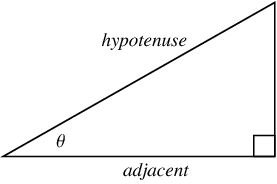
\includegraphics[width=0.35\columnwidth]{pic1.png}
%		\end{center}
		
		In mathematics, the inverse trigonometric functions (also called arcus function, antitrigonometric functions or cyclometric functions) are the inverse of the basic trigonometric functions (Specifically they are the inverse of sine, cosine, tangent, cotangent, secant and cosecant functions) and are used to obtain an angle from any of the angle’s trigonometric ratios. Thus, similar to the definition of cosine, the arccos can be defined as,
		\begin{center}
			\Large arccos $\theta$=\Large$\frac{hypotenuse}{adjacent}$
		\end{center}
	
	\section{Graph, Domain \& Range of arccos(x)}
		arccos(x) is the inverse function of f(x)=cos(x) for 0$\leq$x$\leq$$\pi$. The domain of y=arccos(x) is the range of f(x)=cos(x) for 0$\leq$x$\leq$$\pi$ and given by the interval [-1,1]. The range of arccos(x) is the domain of f which is given by the interval [0,$\pi$].\par
		The graph, domain and range of both cos(x) and arccos(x) is as shown below,
		\begin{center}
			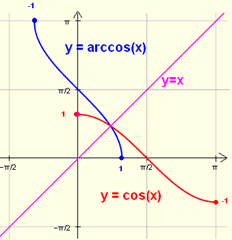
\includegraphics[width=0.35\columnwidth]{pic2.png}
		\end{center}
	
	\section{Arccos table}
	\begin{center}
		\begin{tabular}{c|c|c}
			\hline
			x&arccos(x)&arccos(x)\\
			 &(Rad)&($^{\circ}$)\\
			 \hline
			 -1&$\pi$&180$^{\circ}$\\
			 \hline
			 -$\sqrt{3}$/2&5$\pi$/6&150$^{\circ}$\\
			 \hline
			 -$\sqrt{2}$/2&3$\pi$/4&135$^{\circ}$\\
			 \hline
			 -1/2&2$\pi$/3&120$^{\circ}$\\
			 \hline
			 0&$\pi$/2&90$^{\circ}$\\
			 \hline
			1/2&$\pi$/3&60$^{\circ}$\\
			 \hline
			 $\sqrt{2}$/2&$\pi$/4&45$^{\circ}$\\
			 \hline
			 $\sqrt{3}$/2&$\pi$/6&30$^{\circ}$\\
			 \hline
			 1&0&0$^{\circ}$\\
			 \hline
		\end{tabular}
	\end{center}
	
	\section{References}
		\begin{enumerate}
		\item[i.] http://mathworld.wolfram.com/Cosine.html
		\item[ii.] https://www.analyzemath.com/Graphing/graphing\_arccosine.html
		\item[iii.] https://en.wikipedia.org/wiki/Inverse\_trigonometric\_functions
		\item[iv.] https://www.rapidtables.com/math/trigonometry/arccos.html\#definition
		\end{enumerate}
		
	
		
		
%	\end{flushleft}
	
\end{document}